\fancyhead[LH]{上海交通大学学位论文}
\fancyhead[RH]{第三章\quad 图表、公式格式}
\section{图表、公式格式}
\subsection{图表格式}

\begin{figure}[htb] 
\center{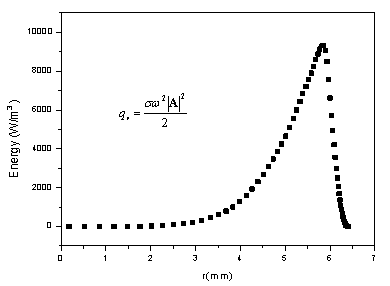
\includegraphics[width=0.95\textwidth]  {fig/fig2.png}} 
\bicaption{内热源沿径向的分布}{Distribution of internal heat sources along the radial direction}
\end{figure}



\begin{table}[!htbp]
    \centering
    \bicaption{高频感应加热的基本参数}{Basic parameters of high frequency induction heating}
    \begin{tabular}{cccc}
    \toprule
    感应频率 &感应发生器功率 & 工件移动速度  &感应圈与零件间隙\\
    (KHz)&($\% \times$80Kw) &(mm/min)  &(mm)\\
    \midrule
    250 &88 &5900 &1.65\\
    250 &88 &5900 &1.65\\
    250 &88 &5900 &1.65\\
    250 &88 &5900 &1.65\\
    \bottomrule
    \end{tabular}
\end{table}


\begin{table}
    \centering
    \begin{tabular}{cccc}
    \multicolumn{4}{l}{\textbf{续表}}
    \vspace{6pt}\\
    \toprule
    感应频率 &感应发生器功率 & 工件移动速度  &感应圈与零件间隙\\
    (KHz)&($\% \times$80Kw) &(mm/min)  &(mm)\\
    \midrule
    250 &88 &5900 &1.65\\
    250 &88 &5900 &1.65\\
    \bottomrule
    \end{tabular}
\end{table}
%表格太大需要转页时,需要在续表上方注明“续表”,表头也应重复排出。


\subsection{公式格式}
\vspace{-10mm}
\begin{eqnarray}
\frac{1}{\mu} \nabla^2A - j \omega \sigma A -\nabla(\frac{1}{\mu}) \times(\nabla \times A)+J_0=0
\end{eqnarray}

\subsection{本章小结}
\begin{figure}[htb] 
    \center{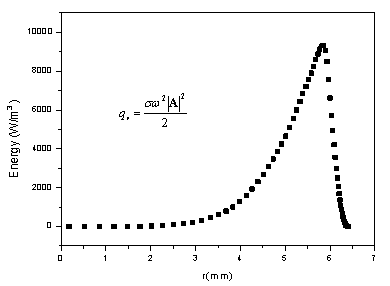
\includegraphics[width=0.95\textwidth]  {fig/fig2.png}} 
    \bicaption{内热源沿径向的分布}{Distribution of internal heat sources along the radial direction}
\end{figure}
本章介绍了……

\clearsection